%!TEX root = ../thesis.tex
%*******************************************************************************
%****************************** Third Chapter **********************************
%*******************************************************************************
\chapter{Experiments}

% **************************** Define Graphics Path **************************
\ifpdf
    \graphicspath{{Chapter3/Figs/Raster/}{Chapter3/Figs/PDF/}{Chapter3/Figs/}}
\else
    \graphicspath{{Chapter3/Figs/Vector/}{Chapter3/Figs/}}
\fi

We compare the accuracy of gMatrix without partitioning and with partitioning for answering edge frequency estimation queries.

\section{Implementation}
The code used for all of the experiments are implemented in C++. All experiments were performed on Intel Xeon 2GHz 16GB server.

We note that some of the variables mentioned in the earlier chapter are made to be constants for the purpose of the project. These include:

\begin{itemize}
\item The data sample used for partitioning is the same in all experiments, i.e. they are only randomly sampled once using Reservoir Sampling \cite{reservoir}. All of the samples' size are 5\% of the corresponding dataset size. They are not regenerated on different runtimes of the experiments.
\item Statistical variance threshold for filtering source nodes to be used for the partitioning algorithm is set to 100 for all experiments.
\item For outlier ratio estimation, data sample is split by 90:10 ratio for all experiments.
\item For the first terminating condition of the sketch partitioning algorithm, the minimum number of rows $w_0$ for any partition is set to 400 in all experiments.
\item For the second terminating condition of the sketch partitioning algorithm, the upper-bound constant $C$ is set to $0.1$ in all experiments.
\end{itemize}

\section{Datasets}
The datasets used for the experiments are the same graph streams used for evaluating gMatrix in \cite{khan}, such as:

\begin{itemize}
\item IP-Trace Network Stream \cite{khan}
\item Twitter Communication Stream \cite{khan}
\item Friendster Stream with Zipf Frequency distribution \cite{khan}
\end{itemize}

All datasets used for all of the experiments consist of distinct edges only.

\section{Metrics}
\subsection{Edge Frequency \& Node Aggregate-Frequency Estimation}
\subsubsection{Observed Error \cite{khan}}
\[
observed\;error = \frac{ \sum_{i=1}^{|Q|}{|\tilde{f}(q_i) - f(q_i)|} }{\sum_{i=1}^{|Q|}f(q_i)}
\]
where $Q = \{q_i\}$ is the set of queries, $\tilde{f}$ is the estimated frequency, and $f$ is the actual frequency.

\subsubsection{Average Relative Error \cite{DBLP}}
\[
average\;relative\;error = \frac{1}{|Q|} \sum_{i=1}^{|Q|} \frac{\tilde{f}(q_i)-f(q_i)}{f(q_i)}
\]
where $Q = \{q_i\}$ is the set of queries, $\tilde{f}$ is the estimated frequency, and $f$ is the actual frequency.

\subsubsection{Effective Queries \cite{DBLP}}
Both Observed Error and Average Relative Error may be biased if the frequencies of the queries vary a lot, so we define queries as "effective" if the relative error is not exceeding $T$. The percentage of effective queries is computed by,
\[
effective\;queries = \frac{|\{q|\frac{\tilde{f}(q)-f(q)}{f(q)} \leq T, q \in Q\}|}{|Q|} \cdot 100\%
\]
where $Q = \{q_i\}$ is the set of queries, $\tilde{f}$ is the estimated frequency, and $f$ is the actual frequency.

In the project, $T$ is a constant and is set to 5, as also is the case in \cite{DBLP}.

\subsection{Heavy Hitter Edge Estimation}
\subsubsection{False Positive Rate \cite{khan}}
The metric measures the percentage of edges that are misclassified as heavy-hitter edges.
\[
false\;positive\;rate(\%) = \frac{#false\;heavyhitter\;edges}{#true\;heavyhitter\;edges} \cdot 100\%
\]

\clearpage
\section{Results}

\subsection{Edge Frequency Estimation}

\paragraph{Friendster dataset}
Partitioning reduces the observed error and the average relative error of the estimations, as seen on figures \ref{fig:F11}-\ref{fig:F21}. The lower errors are possible because partitioning reduces the number of queries with high relative errors (queries $q$ such that $\frac{\tilde{f}(q)-f(q)}{f(q)} > T$), as the number of effective queries themselves are actually lower with partitioning as seen on figure \ref{fig:F31}.

\paragraph{Twitter dataset}
Partitioning does not seem to be effective at all as seen on figures \ref{fig:T11}-\ref{fig:T32}.

\paragraph{IP-Trace dataset}
Partitioning reduces the observed error and the average relative error of the estimations, as seen on figures \ref{fig:I11}-\ref{fig:I21}. Unlike the results on the Friendster dataset, the number of effective queries after partitioning are only significantly lower on $h=1000$ and is actually higher than without partitioning on $h=4000$.

%Friendster
%Observed error

\begin{figure}[!htbp]
\centering
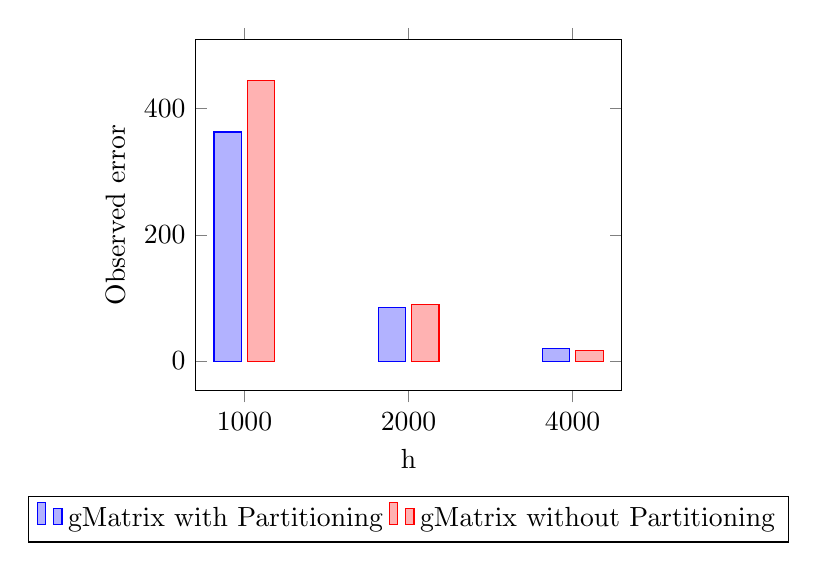
\begin{tikzpicture}
  \begin{axis}[
      ybar,
      enlargelimits=0.15,
      legend style={at={(0.5,-0.3)},anchor=north,legend columns=-1},
      ylabel={Observed error},
      xlabel={h},
      width=7cm,
      symbolic x coords={1000,2000,4000},
      xtick=data
    ]
      \addplot 
	  coordinates {
        (1000,  362.84)
        (2000,  85.24)
        (4000,  19.31)
      };
      \addplot 
	  coordinates {
        (1000,  444.81)
        (2000,  90.16)
        (4000,  17.30)
      };
      \legend{gMatrix with Partitioning,gMatrix without Partitioning}
  \end{axis}
\end{tikzpicture}
\caption{Observed error on Friendster dataset considered over 1 million random edges} \label{fig:F11}
\end{figure}

\begin{figure}[!htbp]
\centering
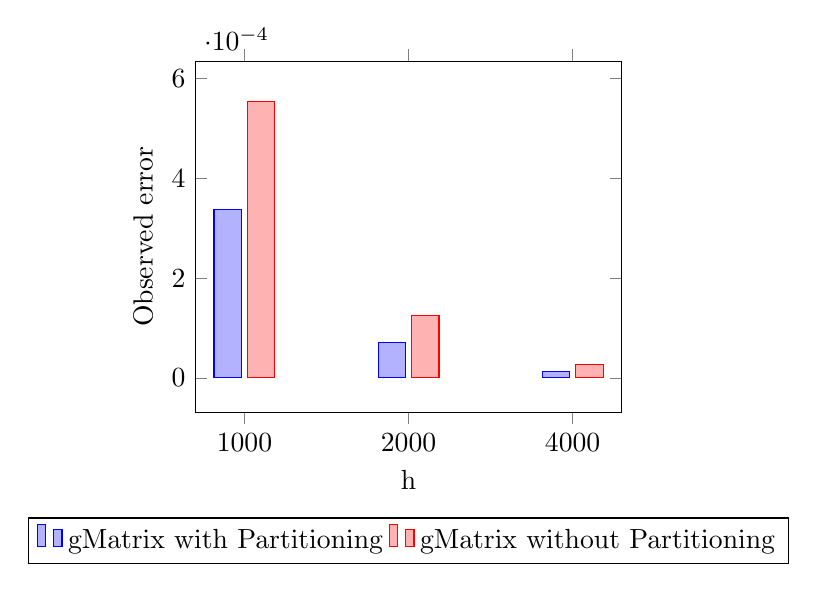
\begin{tikzpicture}
  \begin{axis}[
      ybar,
      enlargelimits=0.15,
      legend style={at={(0.5,-0.3)},anchor=north,legend columns=-1},
      ylabel={Observed error},
      xlabel={h},
      width=7cm,
      symbolic x coords={1000,2000,4000},
      xtick=data
    ]
      \addplot 
	  coordinates {
        (1000,  0.000338304)
        (2000,  7.17931e-05)
        (4000,  1.25923e-05)
      };
      \addplot 
	  coordinates {
        (1000,  0.000553365)
        (2000,  0.000124219)
        (4000,  2.61629e-05)
      };
      \legend{gMatrix with Partitioning, gMatrix without Partitioning}
  \end{axis}
\end{tikzpicture}
\caption{Observed error on Friendster dataset considered over top-500 highest frequency edges} \label{fig:F12}
\end{figure}

% Average relative error

\begin{figure}[!htbp]
\centering
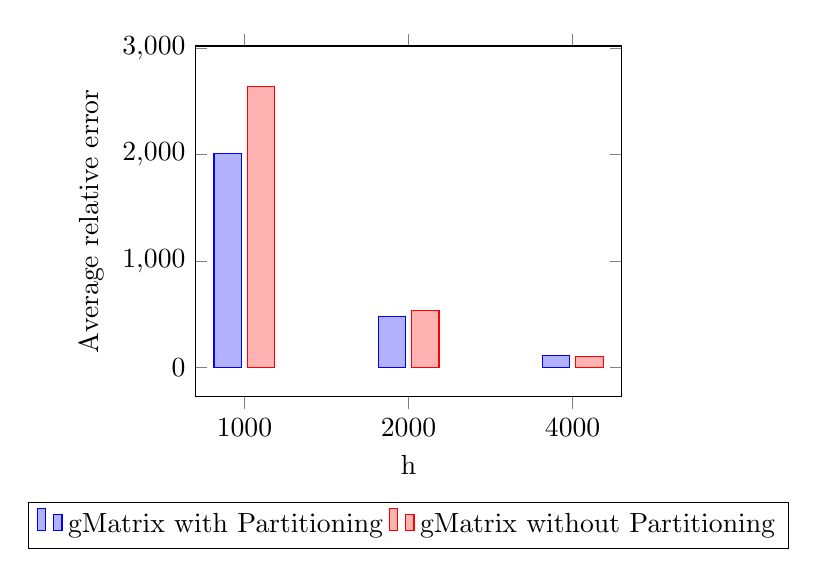
\begin{tikzpicture}
  \begin{axis}[
      ybar,
      enlargelimits=0.15,
      legend style={at={(0.5,-0.3)},anchor=north,legend columns=-1},
      ylabel={Average relative error},
      xlabel={h},
      width=7cm,
      symbolic x coords={1000,2000,4000},
      xtick=data
    ]
      \addplot 
	  coordinates {
        (1000,  2009.98)
        (2000,  478.512)
        (4000,  110.623)
      };
      \addplot 
	  coordinates {
        (1000,  2642.89)
        (2000,  535.386)
        (4000,  102.601)
      };
      \legend{gMatrix with Partitioning,gMatrix without Partitioning}
  \end{axis}
\end{tikzpicture}
\caption{Average relative error on Friendster dataset considered over 1 million random edges} \label{fig:F21}
\end{figure}

\begin{figure}[!htbp]
\centering
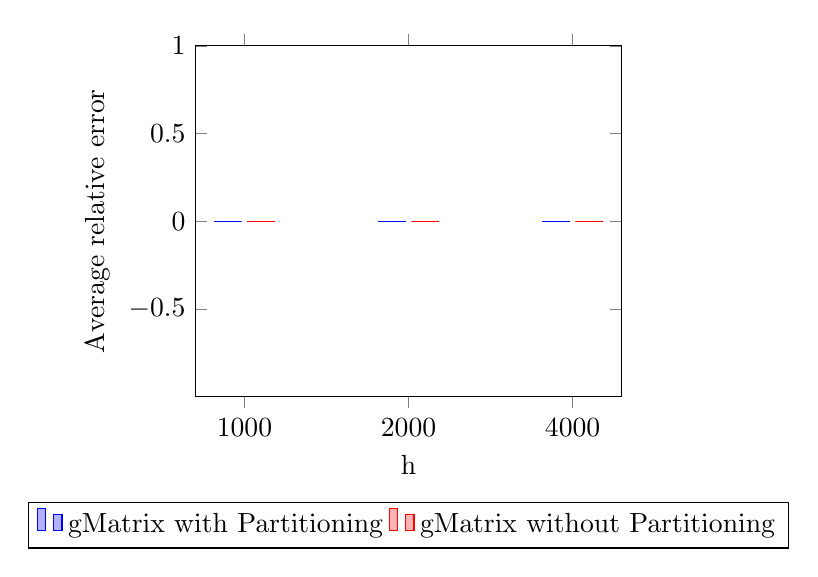
\begin{tikzpicture}
  \begin{axis}[
      ybar,
      enlargelimits=0.15,
      legend style={at={(0.5,-0.3)},anchor=north,legend columns=-1},
      ylabel={Average relative error},
      xlabel={h},
      width=7cm,
      symbolic x coords={1000,2000,4000},
      xtick=data
    ]
      \addplot 
	  coordinates {
        (1000,  0)
        (2000,  0)
        (4000,  0)
      };
      \addplot 
	  coordinates {
        (1000,  0)
        (2000,  0)
        (4000,  0)
      };
      \legend{gMatrix with Partitioning, gMatrix without Partitioning}
  \end{axis}
\end{tikzpicture}
\caption{Average relative error on Friendster dataset considered over top-500 highest frequency edges} \label{fig:F22}
\end{figure}

% Effective queries

\begin{figure}[!htbp]
\centering
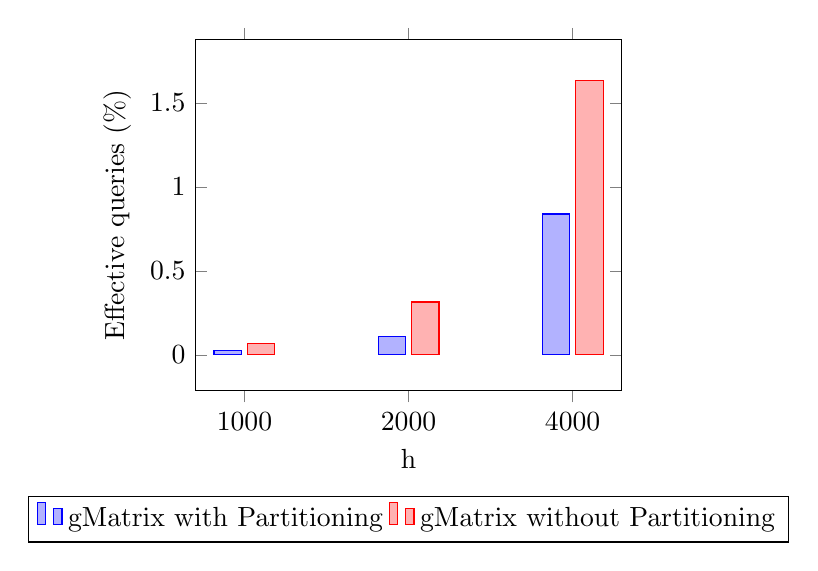
\begin{tikzpicture}
  \begin{axis}[
      ybar,
      enlargelimits=0.15,
      legend style={at={(0.5,-0.3)},anchor=north,legend columns=-1},
      ylabel={Effective queries (\%)},
      xlabel={h},
      width=7cm,
      symbolic x coords={1000,2000,4000},
      xtick=data
    ]
      \addplot 
	  coordinates {
        (1000,  0.0285)
        (2000,  0.1098)
        (4000,  0.8383)
      };
      \addplot 
	  coordinates {
        (1000,  0.0671)
        (2000,  0.3152)
        (4000,  1.6345)
      };
      \legend{gMatrix with Partitioning,gMatrix without Partitioning}
  \end{axis}
\end{tikzpicture}
\caption{Effective queries percentage on Friendster dataset considered over 1 million random edges} \label{fig:F31}
\end{figure}

\begin{figure}[!htbp]
\centering
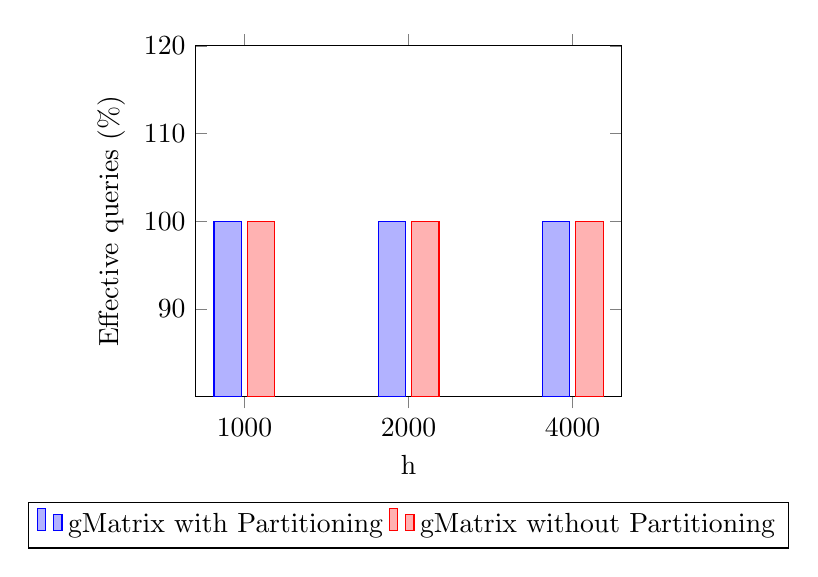
\begin{tikzpicture}
  \begin{axis}[
      ybar,
      enlargelimits=0.15,
      legend style={at={(0.5,-0.3)},anchor=north,legend columns=-1},
      ylabel={Effective queries (\%)},
      xlabel={h},
      width=7cm,
      symbolic x coords={1000,2000,4000},
      xtick=data
    ]
      \addplot 
	  coordinates {
        (1000,  100)
        (2000,  100)
        (4000,  100)
      };
      \addplot 
	  coordinates {
        (1000,  100)
        (2000,  100)
        (4000,  100)
      };
      \legend{gMatrix with Partitioning, gMatrix without Partitioning}
  \end{axis}
\end{tikzpicture}
\caption{Effective queries percentage on Friendster dataset considered over top-500 highest frequency edges} \label{fig:F32}
\end{figure}

%Twitter
%Observed error

\begin{figure}[!htbp]
\centering
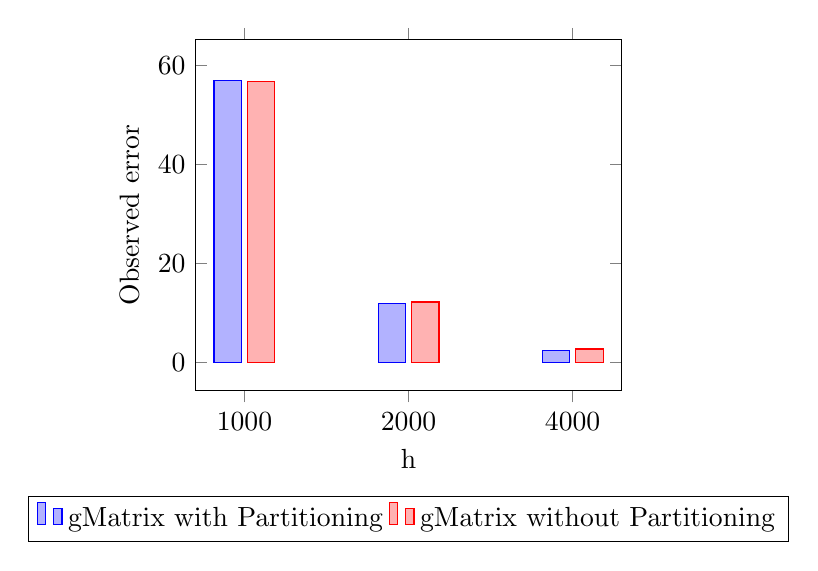
\begin{tikzpicture}
  \begin{axis}[
      ybar,
      enlargelimits=0.15,
      legend style={at={(0.5,-0.3)},anchor=north,legend columns=-1},
      ylabel={Observed error},
      xlabel={h},
      width=7cm,
      symbolic x coords={1000,2000,4000},
      xtick=data
    ]
      \addplot 
	  coordinates {
        (1000,  56.9662)
        (2000,  11.94)
        (4000,  2.4375)
      };
      \addplot 
	  coordinates {
        (1000,  56.7384)
        (2000,  12.1534)
        (4000,  2.67581)
      };
      \legend{gMatrix with Partitioning,gMatrix without Partitioning}
  \end{axis}
\end{tikzpicture}
\caption{Observed error of Twitter dataset considered over 1 million random edges} \label{fig:T11}
\end{figure}

\begin{figure}[!htbp]
\centering
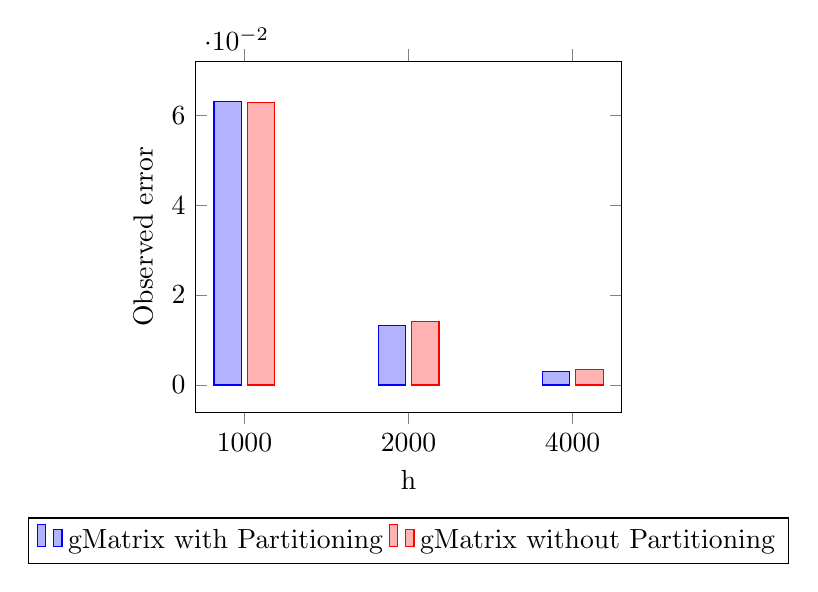
\begin{tikzpicture}
  \begin{axis}[
      ybar,
      enlargelimits=0.15,
      legend style={at={(0.5,-0.3)},anchor=north,legend columns=-1},
      ylabel={Observed error},
      xlabel={h},
      width=7cm,
      symbolic x coords={1000,2000,4000},
      xtick=data
    ]
      \addplot 
	  coordinates {
        (1000,  0.0630049)
        (2000,  0.0132349)
        (4000,  0.00296191)
      };
      \addplot 
	  coordinates {
        (1000,  0.0628949)
        (2000,  0.0140856)
        (4000,  0.00347708)
      };
      \legend{gMatrix with Partitioning, gMatrix without Partitioning}
  \end{axis}
\end{tikzpicture}
\caption{Observed error of Twitter dataset considered over top-500 highest frequency edges} \label{fig:T12}
\end{figure}

% Average relative error

\begin{figure}[!htbp]
\centering
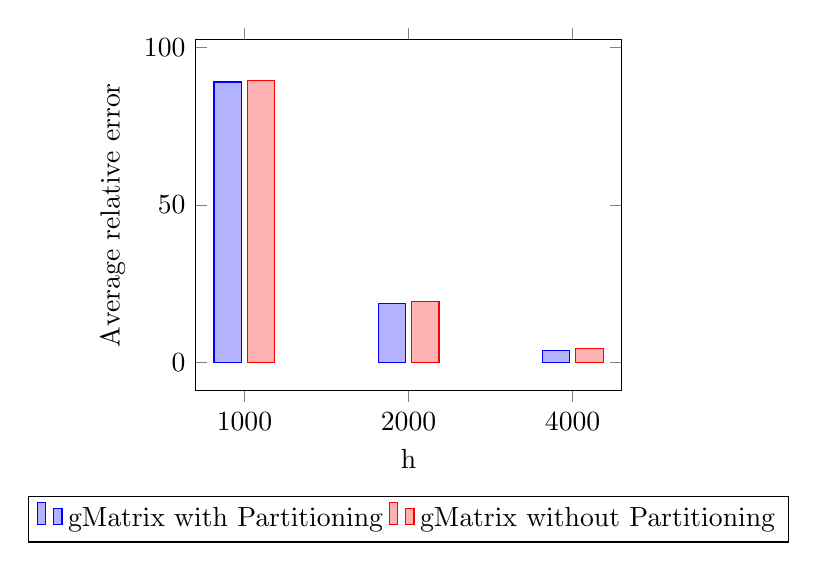
\begin{tikzpicture}
  \begin{axis}[
      ybar,
      enlargelimits=0.15,
      legend style={at={(0.5,-0.3)},anchor=north,legend columns=-1},
      ylabel={Average relative error},
      xlabel={h},
      width=7cm,
      symbolic x coords={1000,2000,4000},
      xtick=data
    ]
      \addplot 
	  coordinates {
        (1000,  88.956)
        (2000,  18.7822)
        (4000,  3.89071)
      };
      \addplot 
	  coordinates {
        (1000,  89.5238)
        (2000,  19.2599)
        (4000,  4.27863)
      };
      \legend{gMatrix with Partitioning,gMatrix without Partitioning}
  \end{axis}
\end{tikzpicture}
\caption{Average relative error on Twitter dataset considered over 1 million random edges} \label{fig:T21}
\end{figure}

\begin{figure}[!htbp]
\centering
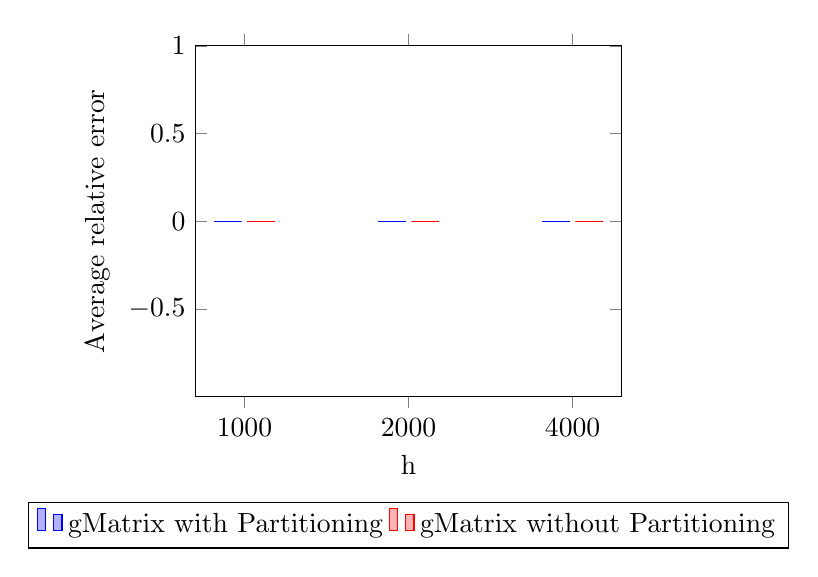
\begin{tikzpicture}
  \begin{axis}[
      ybar,
      enlargelimits=0.15,
      legend style={at={(0.5,-0.3)},anchor=north,legend columns=-1},
      ylabel={Average relative error},
      xlabel={h},
      width=7cm,
      symbolic x coords={1000,2000,4000},
      xtick=data
    ]
      \addplot 
	  coordinates {
        (1000,  0)
        (2000,  0)
        (4000,  0)
      };
      \addplot 
	  coordinates {
        (1000,  0)
        (2000,  0)
        (4000,  0)
      };
      \legend{gMatrix with Partitioning, gMatrix without Partitioning}
  \end{axis}
\end{tikzpicture}
\caption{Average relative error on Twitter dataset considered over top-500 highest frequency edges} \label{fig:T22}
\end{figure}

% Effective queries

\begin{figure}[!htbp]
\centering
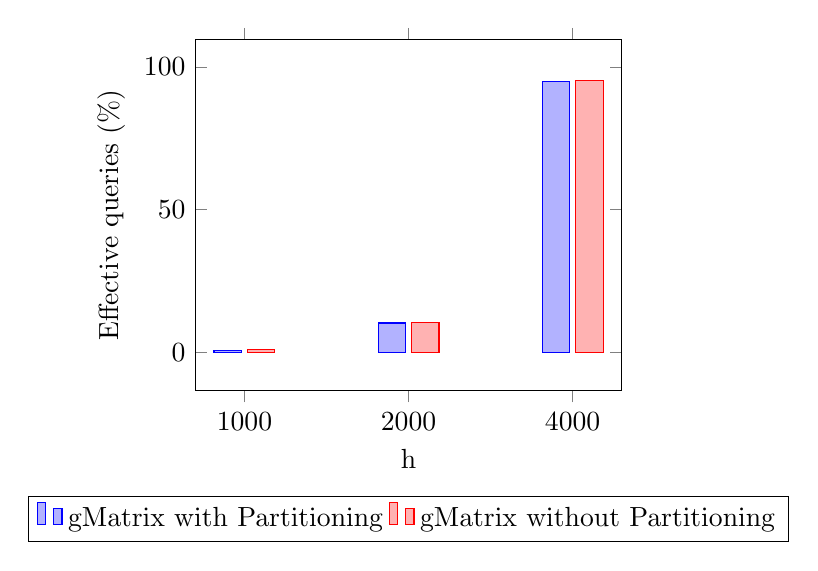
\begin{tikzpicture}
  \begin{axis}[
      ybar,
      enlargelimits=0.15,
      legend style={at={(0.5,-0.3)},anchor=north,legend columns=-1},
      ylabel={Effective queries (\%)},
      xlabel={h},
      width=7cm,
      symbolic x coords={1000,2000,4000},
      xtick=data
    ]
      \addplot 
	  coordinates {
        (1000,  0.6977)
        (2000,  10.214)
        (4000,  94.9675)
      };
      \addplot 
	  coordinates {
        (1000,  0.8046)
        (2000,  10.4912)
        (4000,  95.3025)
      };
      \legend{gMatrix with Partitioning,gMatrix without Partitioning}
  \end{axis}
\end{tikzpicture}
\caption{Effective queries percentage on Twitter dataset considered over 1 million random edges} \label{fig:T31}
\end{figure}

\begin{figure}[!htbp]
\centering
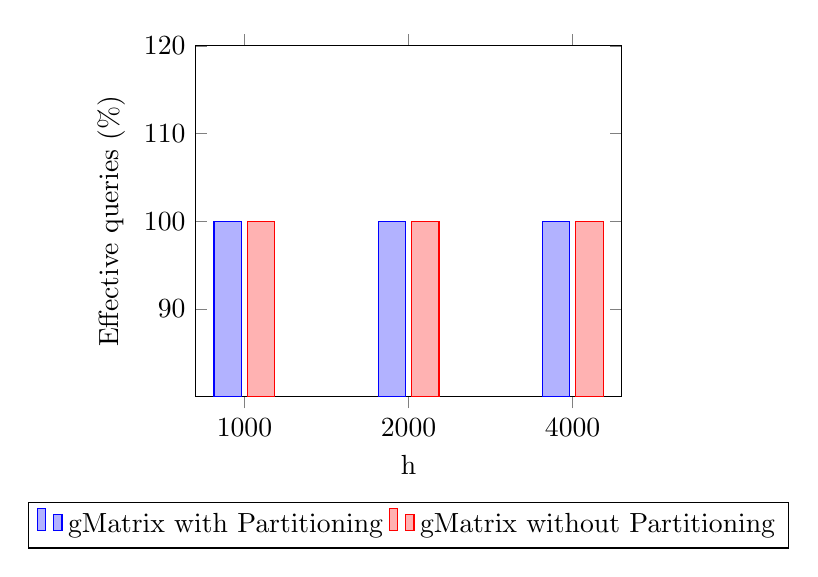
\begin{tikzpicture}
  \begin{axis}[
      ybar,
      enlargelimits=0.15,
      legend style={at={(0.5,-0.3)},anchor=north,legend columns=-1},
      ylabel={Effective queries (\%)},
      xlabel={h},
      width=7cm,
      symbolic x coords={1000,2000,4000},
      xtick=data
    ]
      \addplot 
	  coordinates {
        (1000,  100)
        (2000,  100)
        (4000,  100)
      };
      \addplot 
	  coordinates {
        (1000,  100)
        (2000,  100)
        (4000,  100)
      };
      \legend{gMatrix with Partitioning, gMatrix without Partitioning}
  \end{axis}
\end{tikzpicture}
\caption{Effective queries percentage on Twitter dataset considered over top-500 highest frequency edges} \label{fig:T32}
\end{figure}




%IP Trace
%Observed error
\begin{figure}[!htbp]
\centering
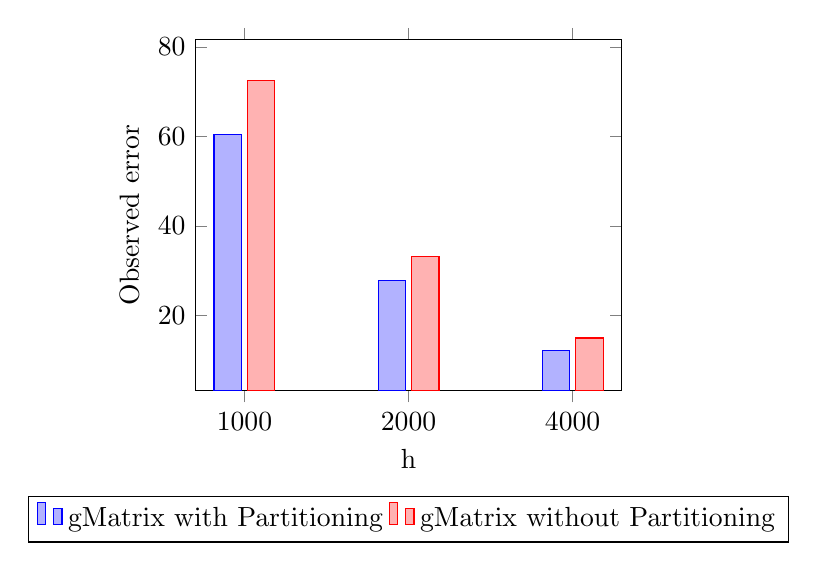
\begin{tikzpicture}
  \begin{axis}[
      ybar,
      enlargelimits=0.15,
      legend style={at={(0.5,-0.3)},anchor=north,legend columns=-1},
      ylabel={Observed error},
      xlabel={h},
      width=7cm,
      symbolic x coords={1000,2000,4000},
      xtick=data
    ]
      \addplot 
	  coordinates {
        (1000,  60.3821)
        (2000,  27.8266)
        (4000,  12.2106)
      };
      \addplot 
	  coordinates {
        (1000,  72.5277)
        (2000,  33.2313)
        (4000,  14.9191)
      };
      \legend{gMatrix with Partitioning,gMatrix without Partitioning}
  \end{axis}
\end{tikzpicture}
\caption{Observed error of IP-Trace dataset considered over 1 million random edges} \label{fig:I11}
\end{figure}

\begin{figure}[!htbp]
\centering
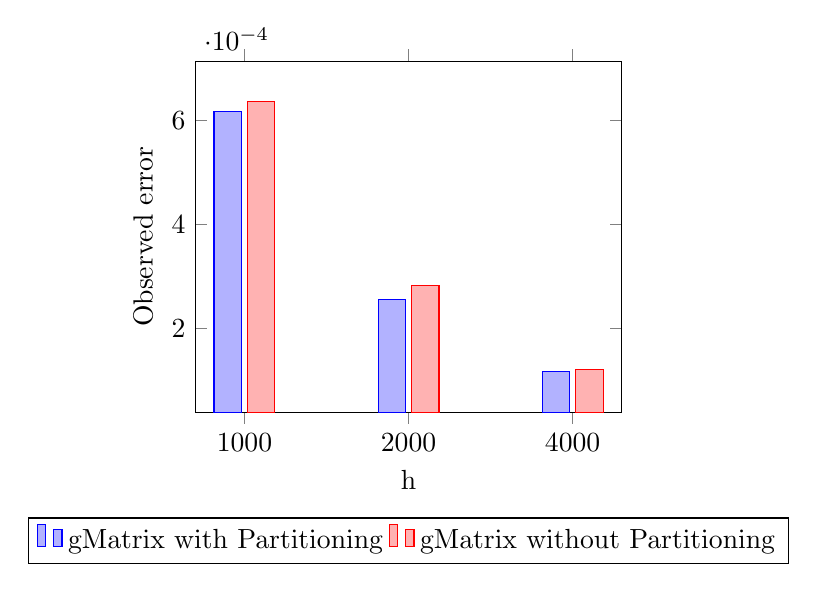
\begin{tikzpicture}
  \begin{axis}[
      ybar,
      enlargelimits=0.15,
      legend style={at={(0.5,-0.3)},anchor=north,legend columns=-1},
      ylabel={Observed error},
      xlabel={h},
      width=7cm,
      symbolic x coords={1000,2000,4000},
      xtick=data
    ]
      \addplot 
	  coordinates {
        (1000,  0.000616909)
        (2000,  0.000255977)
        (4000,  0.000116424)
      };
      \addplot 
	  coordinates {
        (1000,  0.000635283)
        (2000,  0.000282608)
        (4000,  0.000120565)
      };
      \legend{gMatrix with Partitioning, gMatrix without Partitioning}
  \end{axis}
\end{tikzpicture}
\caption{Observed error of IP-Trace dataset considered over top-500 highest frequency edges} \label{fig:I12}
\end{figure}

% Average relative error

\begin{figure}[!htbp]
\centering
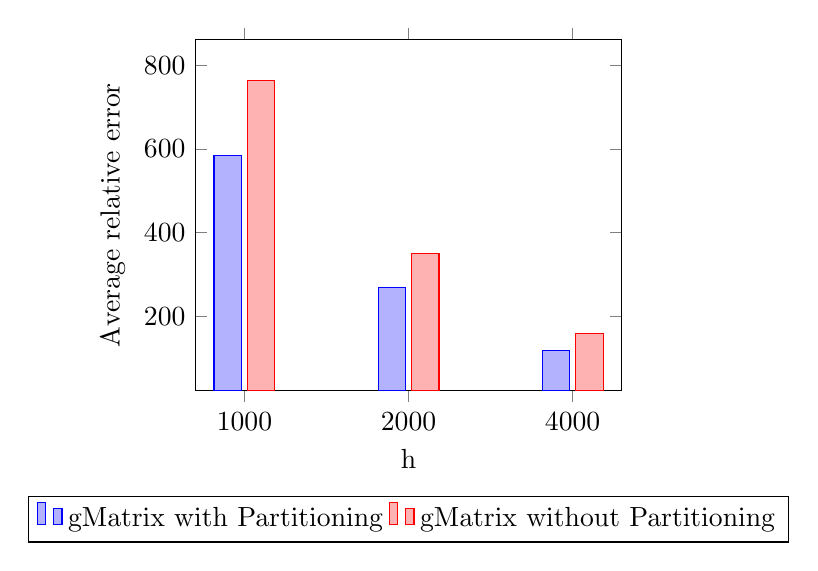
\begin{tikzpicture}
  \begin{axis}[
      ybar,
      enlargelimits=0.15,
      legend style={at={(0.5,-0.3)},anchor=north,legend columns=-1},
      ylabel={Average relative error},
      xlabel={h},
      width=7cm,
      symbolic x coords={1000,2000,4000},
      xtick=data
    ]
      \addplot 
	  coordinates {
        (1000,  583.576)
        (2000,  268.387)
        (4000,  118.987)
      };
      \addplot 
	  coordinates {
        (1000,  764.424)
        (2000,  350.601)
        (4000,  157.765)
      };
      \legend{gMatrix with Partitioning,gMatrix without Partitioning}
  \end{axis}
\end{tikzpicture}
\caption{Average relative error on IP-Trace dataset considered over 1 million random edges} \label{fig:I21}
\end{figure}

\begin{figure}[!htbp]
\centering
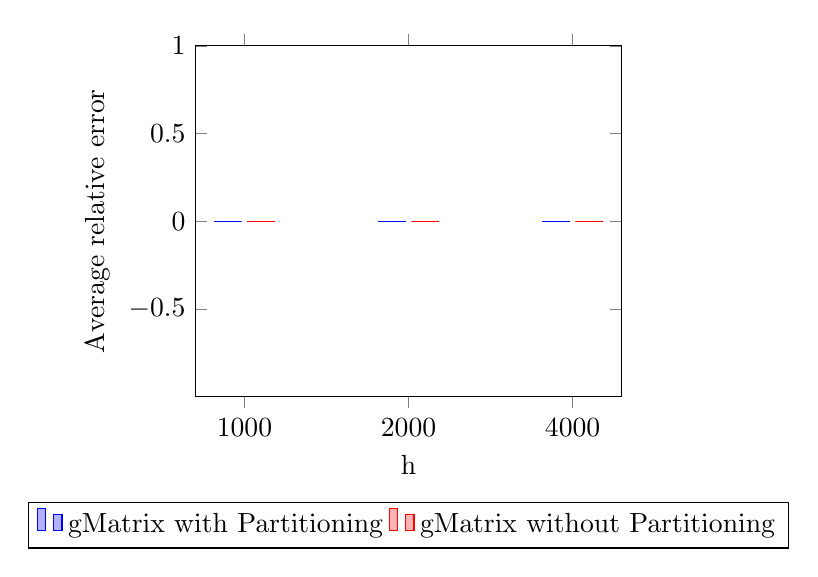
\begin{tikzpicture}
  \begin{axis}[
      ybar,
      enlargelimits=0.15,
      legend style={at={(0.5,-0.3)},anchor=north,legend columns=-1},
      ylabel={Average relative error},
      xlabel={h},
      width=7cm,
      symbolic x coords={1000,2000,4000},
      xtick=data
    ]
      \addplot 
	  coordinates {
        (1000,  0)
        (2000,  0)
        (4000,  0)
      };
      \addplot 
	  coordinates {
        (1000,  0)
        (2000,  0)
        (4000,  0)
      };
      \legend{gMatrix with Partitioning, gMatrix without Partitioning}
  \end{axis}
\end{tikzpicture}
\caption{Average relative error on IP-Trace dataset considered over top-500 highest frequency edges} \label{fig:I22}
\end{figure}

% Effective queries

\begin{figure}[!htbp]
\centering
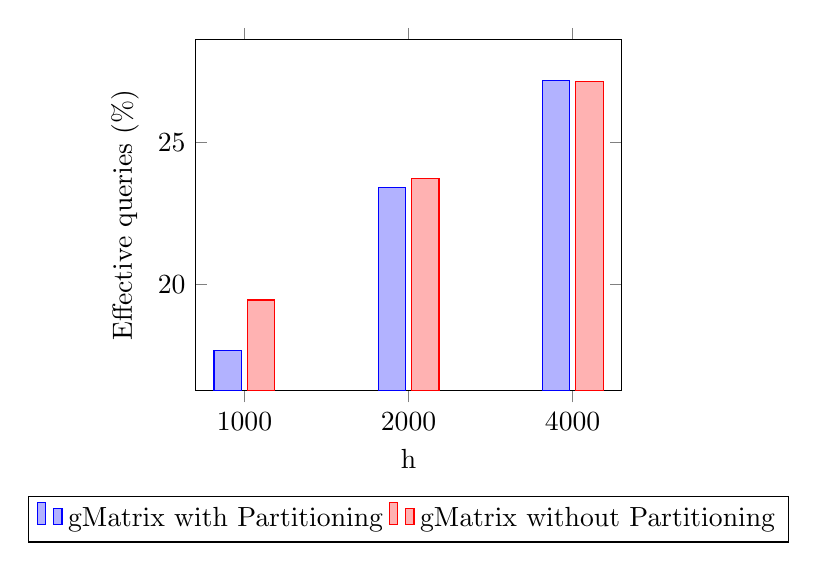
\begin{tikzpicture}
  \begin{axis}[
      ybar,
      enlargelimits=0.15,
      legend style={at={(0.5,-0.3)},anchor=north,legend columns=-1},
      ylabel={Effective queries (\%)},
      xlabel={h},
      width=7cm,
      symbolic x coords={1000,2000,4000},
      xtick=data
    ]
      \addplot 
	  coordinates {
        (1000,  17.6949)
        (2000,  23.426)
        (4000,  27.1898)
      };
      \addplot 
	  coordinates {
        (1000,  19.4597)
        (2000,  23.7307)
        (4000,  27.16)
      };
      \legend{gMatrix with Partitioning,gMatrix without Partitioning}
  \end{axis}
\end{tikzpicture}
\caption{Effective queries percentage on IP-Trace dataset considered over 1 million random edges} \label{fig:I31}
\end{figure}

\begin{figure}[!htbp]
\centering
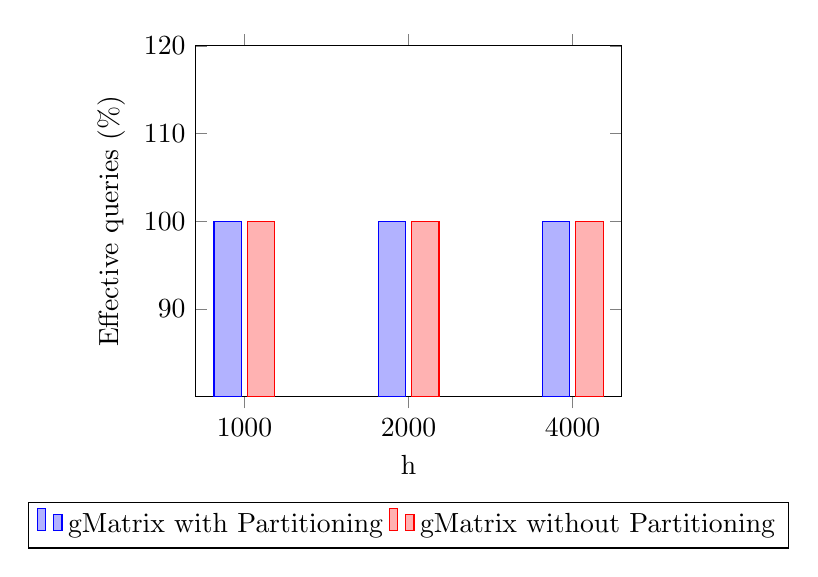
\begin{tikzpicture}
  \begin{axis}[
      ybar,
      enlargelimits=0.15,
      legend style={at={(0.5,-0.3)},anchor=north,legend columns=-1},
      ylabel={Effective queries (\%)},
      xlabel={h},
      width=7cm,
      symbolic x coords={1000,2000,4000},
      xtick=data
    ]
      \addplot 
	  coordinates {
        (1000,  100)
        (2000,  100)
        (4000,  100)
      };
      \addplot 
	  coordinates {
        (1000,  100)
        (2000,  100)
        (4000,  100)
      };
      \legend{gMatrix with Partitioning, gMatrix without Partitioning}
  \end{axis}
\end{tikzpicture}
\caption{Effective queries percentage on IP-Trace dataset considered over top-500 highest frequency edges} \label{fig:I32}
\end{figure}

% Heavy hitter

\clearpage
\subsection{Heavy Hitter Edge Estimation}

Figures \ref{fig:EE1} and \ref{fig:EE2} show that after partitioning, the sketch is more sensitive to low frequency thresholds as the false positive rates are much higher at frequency threshold of 0.01\% of the total stream frequency. However, it performs as good at frequency threshold percentages of 0.1\% and 1\%, with no false positives produced at all.

\begin{figure}[!htbp]
\centering
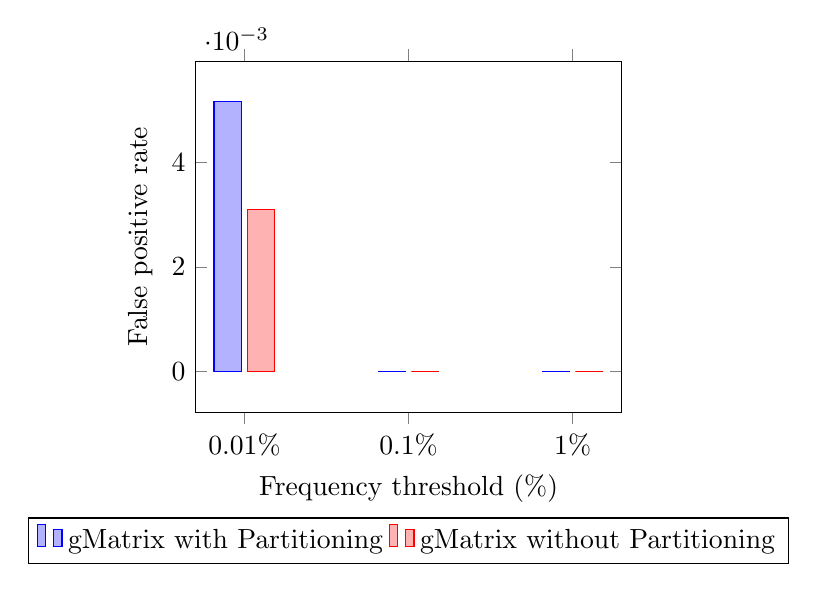
\begin{tikzpicture}
  \begin{axis}[
      ybar,
      enlargelimits=0.15,
      legend style={at={(0.5,-0.3)},anchor=north,legend columns=-1},
      ylabel={False positive rate},
      xlabel={Frequency threshold (\%)},
      width=7cm,
      symbolic x coords={0.01\%,0.1\%,1\%},
      xtick=data
    ]
      \addplot 
	  coordinates {
        (0.01\%,0.00515996)
        (0.1\%, 0)
        (1\%,   0)
      };
      \addplot 
	  coordinates {
        (0.01\%,  0.00309598)
        (0.1\%,   0)
        (1\%,     0)
      };
      \legend{gMatrix with Partitioning, gMatrix without Partitioning}
  \end{axis}
\end{tikzpicture}
\caption{False positive rate of heavy hitter edge estimation on IP-Trace dataset with respect to varying frequency threshold percentages of the total stream frequency} \label{fig:EE1}
\end{figure}

\begin{figure}[!htbp]
\centering
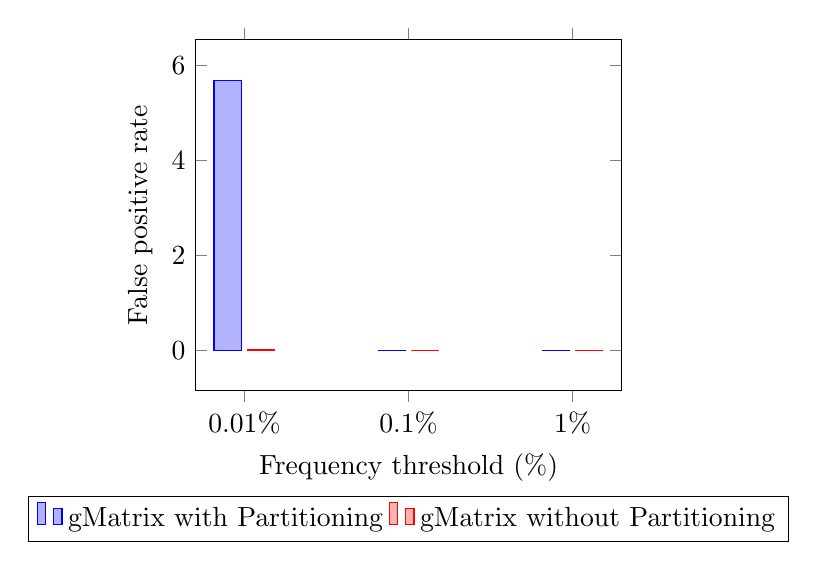
\begin{tikzpicture}
  \begin{axis}[
      ybar,
      enlargelimits=0.15,
      legend style={at={(0.5,-0.3)},anchor=north,legend columns=-1},
      ylabel={False positive rate},
      xlabel={Frequency threshold (\%)},
      width=7cm,
      symbolic x coords={0.01\%,0.1\%,1\%},
      xtick=data
    ]
      \addplot 
	  coordinates {
        (0.01\%,5.691796)
        (0.1\%, 0)
        (1\%,   0)
      };
      \addplot 
	  coordinates {
        (0.01\%,  0.015521)
        (0.1\%,   0)
        (1\%,     0)
      };
      \legend{gMatrix with Partitioning, gMatrix without Partitioning}
  \end{axis}
\end{tikzpicture}
\caption{False positive rate of heavy hitter edge estimation on Friendster dataset with respect to varying frequency threshold percentages of the total stream frequency} \label{fig:EE2}
\end{figure}

%Node Aggregate
\clearpage
\subsection{Node Aggregate-Frequency Estimation}

On the Twitter and IP-Trace dataset, the observed error of source-node aggregate-frequency estimations is lower after partitioning as seen on figure \ref{fig:agg3} and figure \ref{fig:agg5}. However, on the Friendster dataset, figure \ref{fig:agg1} shows that it is higher after partitioning, which is unexpected. According to Theorem \ref{thm:agg1}, an ideal partitioning scheme improves accuracy guarantee, although reduces the probability of the guarantee. We speculate that the higher observed error on the Friendster dataset is due to the high-skewness of the dataset, which makes the partitioning scheme less effective.

Figures \ref{fig:agg2}, \ref{fig:agg4} and \ref{fig:agg6} show the observed error is higher after partitioning in destination-node aggregate-frequency estimations, which is expected since Theorem \ref{thm:agg2} shows that partitioning does not improve the accuracy guarantee itself and only worsens the probability of the guarantee.

\begin{figure}[!htbp]
\centering
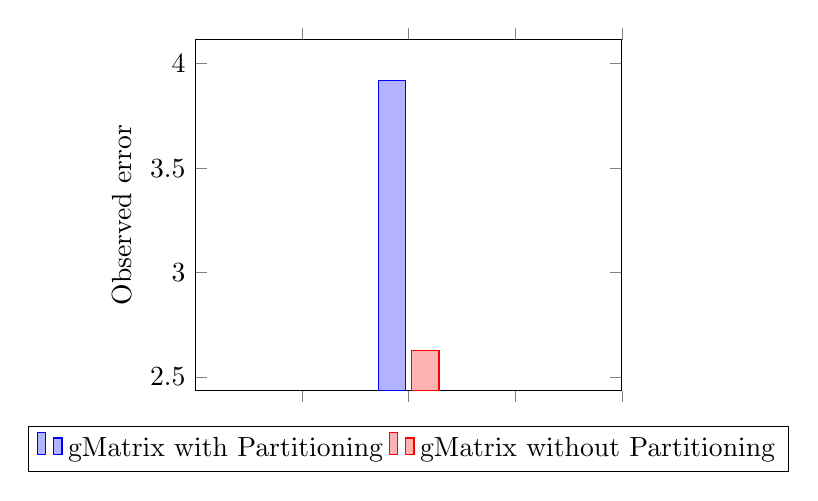
\begin{tikzpicture}
  \begin{axis}[
      ybar,
      enlargelimits=0.15,
      legend style={at={(0.5,-0.1)},anchor=north,legend columns=-1},
      ylabel={Observed error},
      width=7cm,
      xticklabels={,,}
    ]
      \addplot 
	  coordinates {
        (0, 3.920681)
      };
      \addplot 
	  coordinates {
        (0, 2.628615)
      };
      \legend{gMatrix with Partitioning,gMatrix without Partitioning}
  \end{axis}
\end{tikzpicture}
\caption{Observed error of source-node aggregate-frequency queries on top-500 node aggregate-frequencies of the Friendster dataset} \label{fig:agg1}
\end{figure}

\begin{figure}[!htbp]
\centering
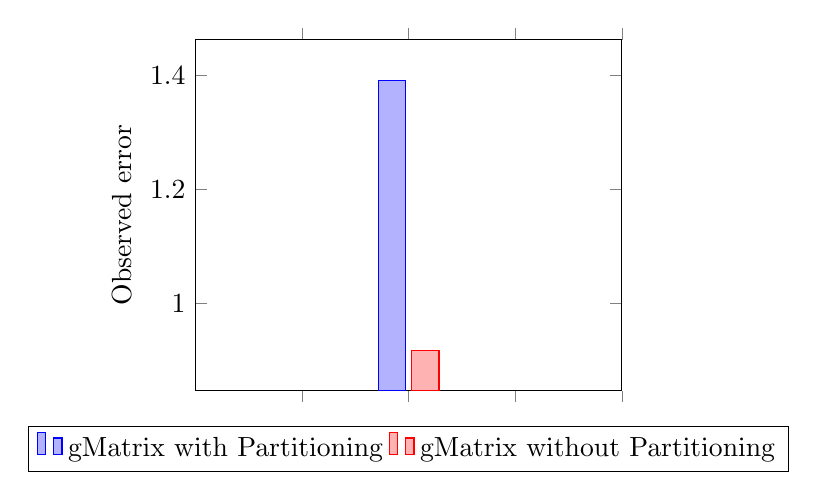
\begin{tikzpicture}
  \begin{axis}[
      ybar,
      enlargelimits=0.15,
      legend style={at={(0.5,-0.1)},anchor=north,legend columns=-1},
      ylabel={Observed error},
      width=7cm,
      xticklabels={,,}
    ]
      \addplot 
	  coordinates {
        (0, 1.391630)
      };
      \addplot 
	  coordinates {
        (0, 0.918388)
      };
      \legend{gMatrix with Partitioning,gMatrix without Partitioning}
  \end{axis}
\end{tikzpicture}
\caption{Observed error of destination-node aggregate-frequency queries on top-500 node aggregate-frequencies of the Friendster dataset} \label{fig:agg2}
\end{figure}

\begin{figure}[!htbp]
\centering
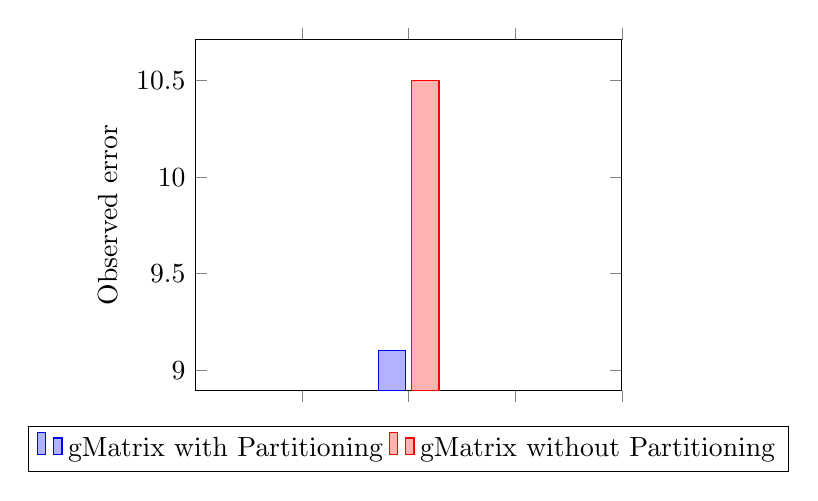
\begin{tikzpicture}
  \begin{axis}[
      ybar,
      enlargelimits=0.15,
      legend style={at={(0.5,-0.1)},anchor=north,legend columns=-1},
      ylabel={Observed error},
      width=7cm,
      xticklabels={,,}
    ]
      \addplot 
	  coordinates {
        (0, 9.104631)
      };
      \addplot 
	  coordinates {
        (0, 10.501604)
      };
      \legend{gMatrix with Partitioning,gMatrix without Partitioning}
  \end{axis}
\end{tikzpicture}
\caption{Observed error of source-node aggregate-frequency queries on top-500 node aggregate-frequencies of the Twitter dataset} \label{fig:agg3}
\end{figure}

\begin{figure}[!htbp]
\centering
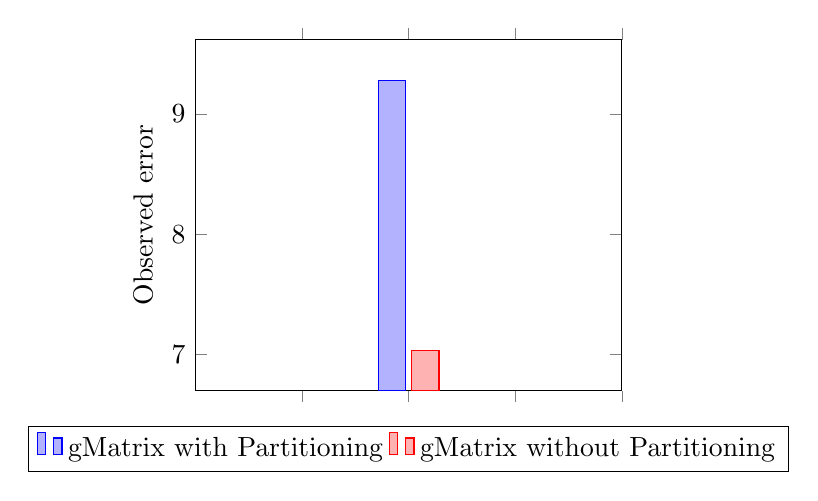
\begin{tikzpicture}
  \begin{axis}[
      ybar,
      enlargelimits=0.15,
      legend style={at={(0.5,-0.1)},anchor=north,legend columns=-1},
      ylabel={Observed error},
      width=7cm,
      xticklabels={,,}
    ]
      \addplot 
	  coordinates {
        (0, 9.279370)
      };
      \addplot 
	  coordinates {
        (0, 7.038425)
      };
      \legend{gMatrix with Partitioning,gMatrix without Partitioning}
  \end{axis}
\end{tikzpicture}
\caption{Observed error of destination-node aggregate-frequency queries on top-500 node aggregate-frequencies of the Twitter dataset} \label{fig:agg4}
\end{figure}


\begin{figure}[!htbp]
\centering
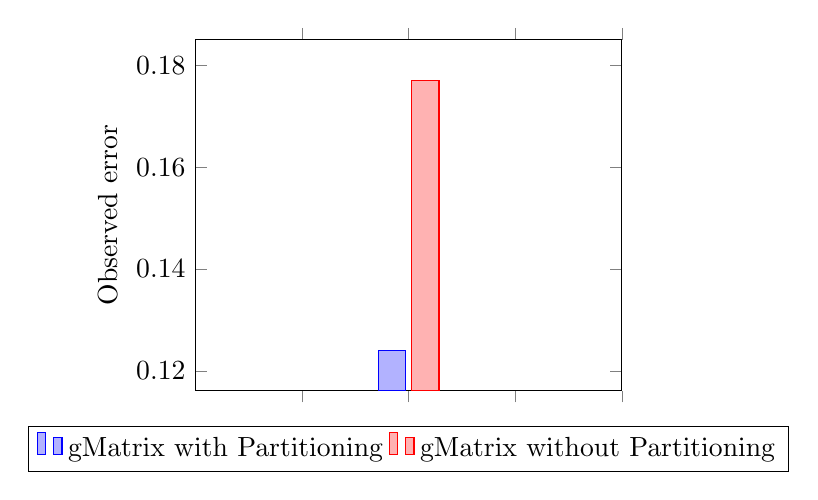
\begin{tikzpicture}
  \begin{axis}[
      ybar,
      enlargelimits=0.15,
      legend style={at={(0.5,-0.1)},anchor=north,legend columns=-1},
      ylabel={Observed error},
      width=7cm,
      xticklabels={,,}
    ]
      \addplot 
	  coordinates {
        (0, 0.124063)
      };
      \addplot 
	  coordinates {
        (0, 0.177073)
      };
      \legend{gMatrix with Partitioning,gMatrix without Partitioning}
  \end{axis}
\end{tikzpicture}
\caption{Observed error of source-node aggregate-frequency queries on top-500 node aggregate-frequencies of the IP-Trace dataset} \label{fig:agg5}
\end{figure}

\begin{figure}[!htbp]
\centering
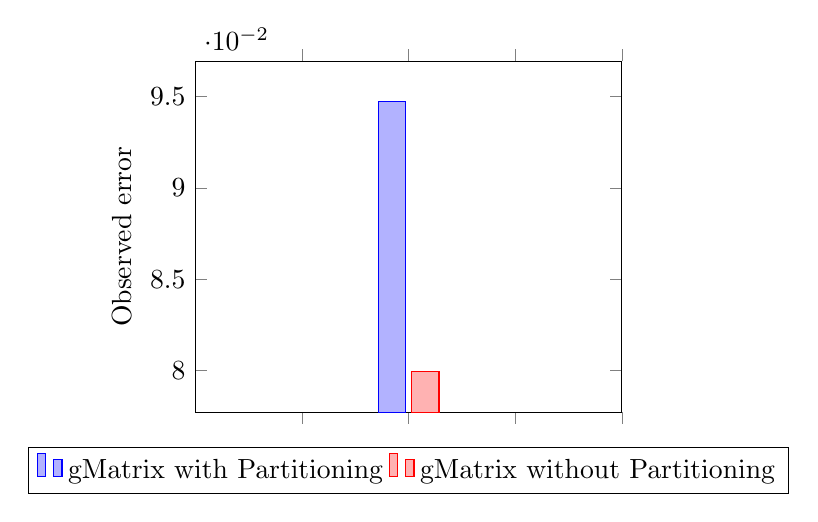
\begin{tikzpicture}
  \begin{axis}[
      ybar,
      enlargelimits=0.15,
      legend style={at={(0.5,-0.1)},anchor=north,legend columns=-1},
      ylabel={Observed error},
      width=7cm,
      xticklabels={,,}
    ]
      \addplot 
	  coordinates {
        (0, 0.094721)
      };
      \addplot 
	  coordinates {
        (0, 0.079930)
      };
      \legend{gMatrix with Partitioning,gMatrix without Partitioning}
  \end{axis}
\end{tikzpicture}
\caption{Observed error of destination-node aggregate-frequency queries on top-500 node aggregate-frequencies of the IP-Trace dataset} \label{fig:agg6}
\end{figure}
